\documentclass[11pt,a4paper,oneside,french,svgnames]{report}
\usepackage[utf8]{inputenc} % force the use of utf8
\usepackage[T1]{fontenc} % font encoding, allows accents
\usepackage[papersize={21cm,29.7cm},top= 2.5cm,bottom=2.5cm, inner=2.5cm, outer=2.5cm]{geometry} % page formatting
\usepackage[francais]{babel} % translate everything in the desired language: table of contents, etc. 'english' can be replaced with 'francais'
\usepackage{graphicx} % images management
\usepackage{wrapfig} % floating images
\usepackage{array} % allow arrays
\usepackage{fancyhdr} % headers/footers management (overrides empty, plain and headings)
\usepackage{listings} % code insertion (MUST BE WRITTEN AFTER BABEL)
%\usepackage[nottoc,numbib]{tocbibind} % bib in toc
%\usepackage{pdfpages} % include PDF documents
\usepackage{enumitem} % for /setlist
\usepackage{color,soul} % add some colors and hightlight
\usepackage{xcolor} % more colors
\usepackage[hyphens]{url} % auto break lines in URL
\usepackage[hidelinks,  colorlinks  = true, % no borders, colors enabled
                        anchorcolor = blue,
                        linkcolor   = black, % links in table of contents
                        urlcolor    = blue,
                        citecolor   = blue]{hyperref}
%\usepackage[%nonumberlist,% no page number
%            toc,% displayed in toc
%            numberedsection,% displayed as a numbered section in toc
%            xindy]{glossaries} % glossary with xindy style. MUST BE WRITTEN AFTER HYPERREF
%\setglossarystyle{listgroup}

\sethlcolor{cyan} % package soul
\newcommand{\file}[1]{\hl{\emph{#1}}} % highlight a file URI

%\makeglossaries
%\loadglsentries{glossary.tex}

%%%%%%%%%%%%%%%%%%%%%%%%%%%%%%%%%%%%%%%%%%%%%%%%%%%%%%%% LISTINGS %%%%%%%%%%%%%%%%%%%%%%%%%%%%%%%%%%%%%%%%%%%%%%%%%%%%%%%%
\definecolor{comment}{rgb}{0.12, 0.38, 0.18 } % adjusted, in Eclipse: {0.25, 0.42, 0.30 } = #3F6A4D
\definecolor{keyword}{rgb}{0.37, 0.08, 0.25}  % #5F1441
\definecolor{string}{rgb}{0.06, 0.10, 0.98} % #101AF9

\lstset{
  language=C++,
  columns=flexible, %prevent extra spaces
  rulecolor=\color{black!50},
  backgroundcolor = \color{blue!10},
  numbers=none, % line numbering
  showspaces=false,
  showtabs=false,
  tabsize=4,
  breaklines=true,
  showstringspaces=false,
  breakatwhitespace=false,
  commentstyle=\color{comment},
  keywordstyle=\color{keyword},
  stringstyle=\color{string},
  basicstyle=\ttfamily,
  extendedchars=true,
  emph=[2]{In},
  emphstyle=[2]\color{black!70},
  morecomment=[l][\color{blue}]{Out},
  frame=single,
  frameround=tttt,
  framerule=0.3pt,
  framesep=4pt,
  belowcaptionskip=2.1pt,
  literate={à}{{\`a }}1 {â}{{\^a}}1 %                         letter a
           {À}{{\`A}}1 {Â}{{\^A}}1 %                         letter A
           {ç}{{\c{c}}}1 %                                   letter c
           {Ç}{{\c{C}}}1 %                                   letter C
           {é}{{\'e}}1 {è}{{\`e}}1 {ê}{{\^e}}1 {ë}{{\"e}}1 % letter e
           {É}{{\'E}}1 {È}{{\`E}}1 {Ê}{{\^E}}1 {Ë}{{\"E}}1 % letter E
           {î}{{\^i}}1 {ï}{{\"i}}1 %                         letter i
           {Î}{{\^I}}1 {Ï}{{\"I}}1 %                         letter I
           {ô}{{\^o}}1 %                                     letter o
           {Ô}{{\^O}}1 %                                     letter O
           {œ}{{\oe}}1 %                                     letter oe
           {Œ}{{\OE}}1 %                                     letter OE
           {ù}{{\`u}}1 {û}{{\^u}}1 {ü}{{\"u}}1 %             letter u
           {Ù}{{\`U}}1 {Û}{{\^U}}1 {Ü}{{\"U}}1 %             letter U
  % above is a hack to force UTF8 compatibility (only for french)
}

% Usage : \code{main.cpp}{C++}
\newcommand{\code}[2]{\lstset{
  language=#2,
  title={{\setlength{\fboxsep}{1pt}\fcolorbox{orange}{yellow!20}{\sffamily\scriptsize
              \textcolor{gray!10}{\_}{#1}\textcolor{gray!10}{\_}}}}
  }
}
%%%%%%%%%%%%%%%%%%%%%%%%%%%%%%%%%%%%%%%%%%%%%%%%%%%%%%%%%%%%%%%%%%%%%%%%%%%%%%%%%%%%%%%%%%%%%%%%%%%%%%%%%%%%%%%%%%%%%%%%%%%

%\parindent=20pt
\fancypagestyle{plain}{
    % Headers
    \fancyhead[R]{Rapport de projet - Printemps 2015}
    \fancyhead[L]{LO21}

    % Footers
    \renewcommand{\footrulewidth}{0.1pt}
    \fancyfoot[C]{Université de Technologie de Compiègne}
    \fancyfoot[LE]{\ifnum\thepage>0 \thepage \fi}
    \fancyfoot[RO]{\ifnum\thepage>0 \thepage \fi}
}

\fancypagestyle{empty}{%
    \renewcommand{\headrulewidth}{0pt} % No sub line
    \fancyhead{} % Empty the header

    \renewcommand{\footrulewidth}{0pt}
    \fancyfoot{}
} 

\setlist[itemize,2]{label={$\bullet$}} % use bullets for nested itemize

% First page
\newcommand{\presentation}[1]{\vspace{0.3cm}\large{\textbf{#1}}\vspace{0.3cm}\\}
\newcommand{\presentationLarge}[1]{\vspace{0.3cm}\LARGE{\textbf{#1}}\vspace{0.3cm}\\}

% Overrides chapter (numbered and no-numbered) headings: remove space, display only the title
\makeatletter
  \def\@makechapterhead#1{%
  \vspace*{0\p@}% avant 50
  {\parindent \z@ \raggedright \normalfont
    %\ifnum \c@secnumdepth >\m@ne
    %    \huge\bfseries \@chapapp\space \thechapter
    %    \par\nobreak
    %    \vskip 20\p@
    %\fi
    \interlinepenalty\@M
    \Huge \bfseries \thechapter\quad #1   
    \vskip 40\p@
  }}
  \def\@makeschapterhead#1{%
  \vspace*{0\p@}% before 50
  {\parindent \z@ \raggedright
    \normalfont
    \interlinepenalty\@M
    \Huge \bfseries  #1\par\nobreak
    \vskip 40\p@
  }}
\makeatother

\newcommand{\ignore}[1]{} % inline comments

\pagenumbering{arabic}
%\addtocounter{page}{-7} % page numbering starts at 1 + (-7)
\pagestyle{plain} % uses fancy

\title{Rapport de projet - P2015 - LO21}
\author{Romain PELLERIN et Lila SINTES}
\date\today

%\setcounter{tocdepth}{4}

\begin{document}
\thispagestyle{empty} % only for the current page

\begin{center}

\includegraphics[height=3cm]{assets/UTC_logo.png}\\
\vspace{2.5cm}
\presentation{Université de Technologie de Compiègne} 
\presentation{LO21}

\vspace{2cm}
\noindent\fbox{
\begin{minipage}{0.9\textwidth}
\begin{center}
    \presentationLarge{Rapport de projet}
    \presentationLarge{\Huge{ProjectCalendar}}
\end{center}
\end{minipage}}
\vspace{3cm}

\presentation{Printemps 2015}
\vspace{1cm}

\def\arraystretch{1.5} % 1 is the default
\begin{tabular}{|>{\hfill\arraybackslash}p{5cm}|p{5cm}|}
\hline
    \multicolumn{2}{|c|}{Romain \textsc{PELLERIN} - Lila \textsc{SINTES}}\\
\hline
     \multicolumn{2}{|c|}{Groupe du mardi après-midi}\\% dates
\hline
    \multicolumn{2}{|c|}{\textit{\today}}\\% dates
\hline
\end{tabular}
\end{center}

\tableofcontents

\chapter{Introduction}
\section{Résumé}
L'objectif de ce TP est d'écrire un programme permettant la gestion d'une ludothèque composée de jeux de société. Un jeu de société est décrit par une fiche contenant les informations suivantes :
\begin{itemize}
  \item Nom du jeu
  \item Genre du jeu : PLATEAU, RPG, COOPERATIF, AMBIANCE ou HASARD
  \item Le nombre de joueurs minimum
  \item Le nombre de joueurs maximum
  \item La durée moyenne d'une partie en minutes
\end{itemize}

\section{Structuration du projet}
Nous avons choisi de structuer notre projet en 5 fichiers pour une meilleure clarté, selon les deux entités principales que sont les \textbf{ludothèques} et les \textbf{jeux} :

\begin{itemize}
  \item \textbf{main.c} Le fichier source contenant le programme principal
  \item \textbf{ludotheque.h} Le fichier d'en-tête contenant les déclarations des structures et fonctions d'une ludothèque
  \item \textbf{ludotheque.c} Le fichier source contenant la définition de chaque fonction d'une ludothèque
  \item \textbf{jeu.h} Le fichier d'en-tête contenant les déclarations des structures et fonctions d'un jeu
  \item \textbf{jeu.c} Le fichier source contenant la définition de chaque fonction d'un jeu
\end{itemize}

\section{Code source}
Le code source est fourni dans l'archive ZIP contenant ce rapport.
\chapter{Implémentation}

\section{Classes métiers}

Ayant un UML à disposition, nous avons par la suite commencé le projet en créant les classes métiers, qui sont en fait les implémentations des entités UML. Par rapport à l'UML, nous avons ajouté les constructeurs, les \textit{getters} et \textit{setters}, les attributs implicites sur l'UML (par exemple, un \lstinline{std::vector} pour les compositions), etc. Voici un extrait de la classe \lstinline{Projet} :

\code{projet.h}{C++}
\begin{lstlisting}
class Projet {
    QString nom;
    QDate dateDisponibilite;
    vector<Tache*> taches;

public:
    Projet(QString m_nom, QDate m_dispo): nom(m_nom), dateDisponibilite(m_dispo){}

    void ajouterTache(Tache *t);

    /**
     * @brief getEcheance permet de connaitre l'échéance du projet
     * @return la date d'échéance la plus éloignée, de l'ensemble des tâches du projet
     */
    QDate getEcheance() const;

    // Getters
    QString getNom() const {return nom;}
    QDate getDispo() const {return dateDisponibilite;}

    // Setters
    void setNom(const QString& m_nom) {nom = m_nom;}
    void setDispo(const QDate& m_dateDispo) {dateDisponibilite  = m_dateDispo;}

    ~Projet();
};
\end{lstlisting}

Nous avons choisi d'utiliser \textbf{trois singletons} pour les tâches, les projets et les événements (programmations) de l'agenda. Ces trois types d'entités seront respectivement contenu dans des \lstinline{TacheManage}, \lstinline{ProjetManager} et \lstinline{EvenementManager}. Cela permet d'accéder aux même objets, depuis n'importe quelle classe de l'application.

\section{Classes des interfaces graphiques}
Lors de la création des interfaces graphiques avec Qt, les classes minimales sont générées (constructeur et destructeur). Nous avons donc rajouté des méthodes pour effectuer certaines actions, comme par exemple :
\begin{itemize}
  \item Des signaux et slots pour réagir à des clics sur des éléments graphiques
  \item Des méthodes qui rafraîchissent l'ensemble de l'interface graphique
\end{itemize}

\section{Fonction \lstinline{main()}}
Notre fonction \lstinline{main()} joue un rôle très important dans l'application. Voici dans l'ordre ce qu'elle fait :
\begin{enumerate}
  \item \textbf{Instanciation des trois singletons.}
  \item \textbf{Création (si non présent) du fichier de la base SQLite dans un sous-répertoire propre à notre application, dans le répertoire de l'utilisateur.}
  \item \textbf{Connexion à la base et vérification que les tables nécessaires existent, sinon la table est \og re-initiliasée\fg{}.} Pour pouvoir faire évoluer l'application et la base facilement, il conviendrait d'avoir une table qui contient le numéro de version de l'application. Ainsi, lors des mises à jour de l'application, il serait aisé de savoir s'il faut recréer la base de données ou non.
  \item \textbf{Chargement dans les trois singletons des projets, tâches et événements contenus en base de données.}
  \item \textbf{Affichage de la fenêtre graphique.}
\end{enumerate}

\bigskip

Les différentes exceptions qui peuvent survenir sont gérées par des blocs \lstinline{try/catch} avec affichage des messages d'erreurs à l'utilisateur via une \textit{pop-up}. Par exemple :

\code{main.cpp}{C++}
\begin{lstlisting}
try {
    em->setDatabase(&sdb); // em = EvenementManager::getInstance()
    em->loadEvents();
} catch (EvenementManagerException& e) {
    fenetre.showError("Project Calendar", e.getInfo());
    app.exit(0);
    return 0;
}
\end{lstlisting}
\code{mainwindow/h}{C++}
\begin{lstlisting}
void showError(QString titre, QString description) {
    QMessageBox::warning(this, titre, description);
}
\end{lstlisting}
\chapter{Fonctionnalités}

\noindent Voici le rendu visuel de l'application, composé de deux contenus principaux, accessible via des onglets :

\begin{figure}[h!]
  \centering
    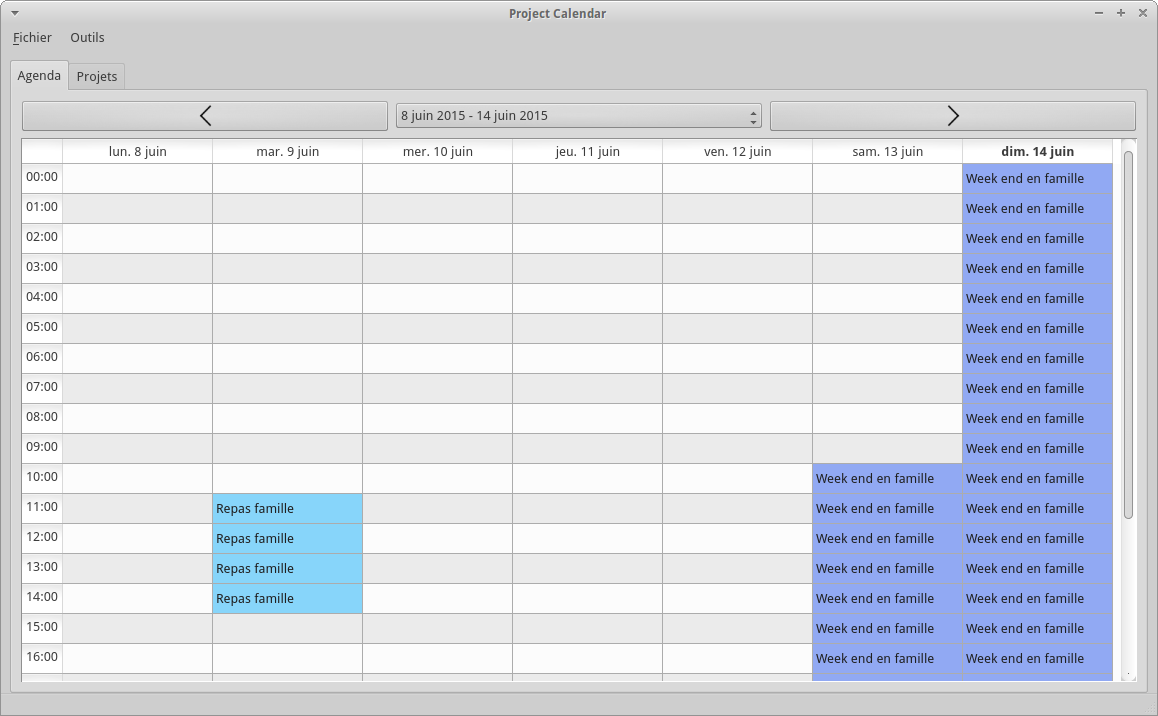
\includegraphics[width=1.0\textwidth]{assets/screen_agenda.png}
    \caption{Partie de l'application dédiée à l'agenda}
\end{figure}

\begin{figure}[h!]
  \centering
    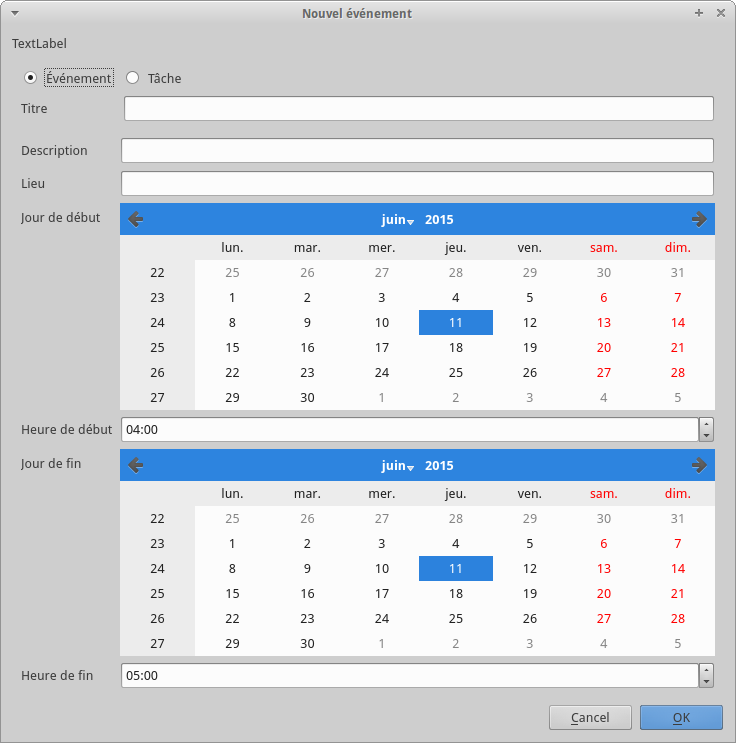
\includegraphics[width=0.49\textwidth]{assets/screen_event.png}
    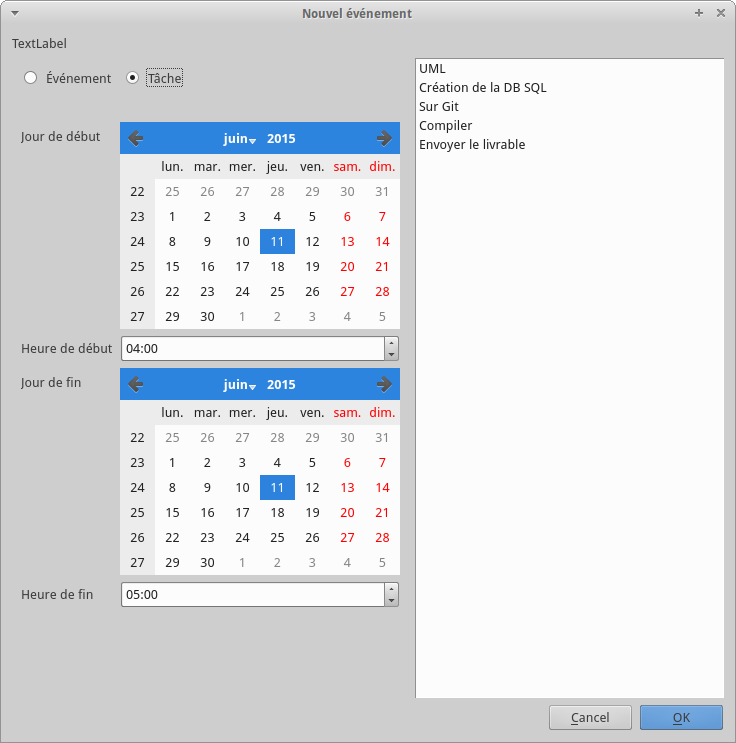
\includegraphics[width=0.49\textwidth]{assets/screen_event_tache.png}
    \caption{Création d'un nouvel événement}
\end{figure}

\begin{figure}[h!]
  \centering
    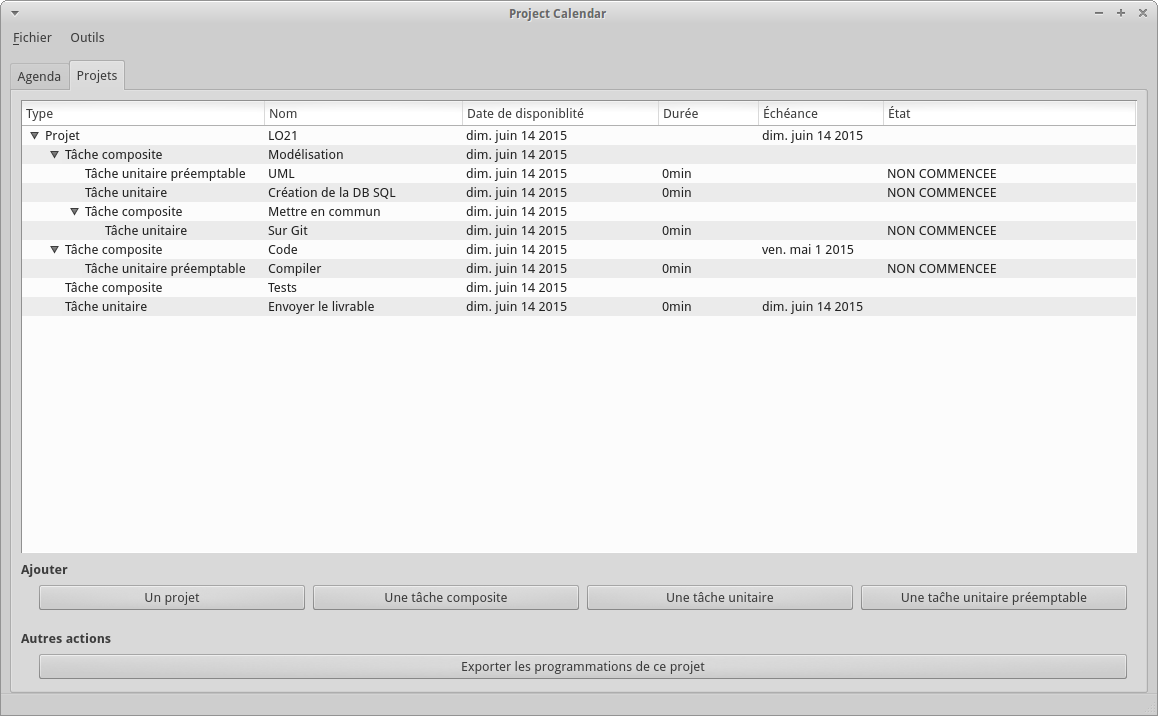
\includegraphics[width=1.0\textwidth]{assets/screen_projets.png}
    \caption{Partie de l'application dédiée aux projets et tâches}
\end{figure}

Nous avons implémenté les fonctionnalités suivantes.

\section{Choix de la semaine à afficher}

Par défaut, la semaine courante est affichée. Le jour courant est en gras. L'utilisateur peut changer la semaine affichée à l'aide d'une liste déroulante (au milieu de l'écran) ou à l'aide des boutons \og Suivant\fg{} et \og Précédent\fg{}.

L'agenda affiche les événements programmée pour la semaine affichée.

\section{Création}
\subsection{D'un événement (une programmation)}

Un clic sur un case de l'agenda permet de programmer un événement (les champs dates et heures sont pré-remplis en fonction de la case cliquée). Des vérifications sont faites (par exemple, un événement doit finir après sa date et heure de début)

\subsection{D'un projet}

Via l'onglet \og Projets\fg{}, l'utilisateur peut créer un nouveau projet.

\subsection{D'une tache composite, unitaire ou unitaire et préemptable}

De la même façon qu'un projet, l'utilisateur peut créer les trois type de tâches. Néanmoins, il doit au préalable avoir sélectionné le projet ou la tâche composite qui va accueillir la nouvelle tâche. Les tâches composites ne peuvent être contenus que dans des projets ou des tâches composites. Les éléments de \og\textit{top-level}\fg{} sont donc les projets.

\section{Modification}

Les attributs des projets et tâches peuvent être modifiés (la durée d'une tâche unitaire par exemple).

\section{Export XML}
\subsection{De la semaine actuellement affichée}

Il est possible, via le menu, d'exporter l'ensemble des programmations de la semaine couramment affichée dans un fichier XML.

\subsection{Des programmations relatives aux tâches d'un projet donné}

On peut également exporter uniquement les événements (tâches programmées) d'un projet selectionné, via un bouton en bas, sur l'interface des projets.

\section{Suppression}

Il est possible via le menu de supprimer soit l'ensemble des événements, soit l'ensemble des tâches et projets. La suppressions d'une tâche entraîne la suppression de sa programmation, s'il y en a une.
\chapter{Code}

\section{Design Pattern}
\noindent Nous avons utilisé les \textit{patterns} suivants dans notre projet :
\begin{itemize}
  \item Iterator (sur des \lstinline{std::vector})
  \item Singleton (pour \lstinline{Tache}, \lstinline{Projet} et \lstinline{Evenement})
  \item Composite (une tâche composite contient d'autre tâches, composites ou unitaires)
  \item Factory (seul \lstinline{TacheManager} peut créer des \lstinline{Tache}, les constructeurs sont privés)
  \item Adapter (autour de \lstinline{std::vector})
\end{itemize}

\section{Évolutivité}
Nous n'avons pas trouvé l'usage des \textit{templates}, étant donné que nous utilisons la classe abstraite \lstinline{Tache}, qui contient des méthodes virtuelles pures, et dont toutes les tâches héritent. En cela, l'application peut être difficilement maintenable sur certains aspects.

\medskip

Nous aurions pu utiliser des \textit{templates} pour une classe-mère \lstinline{Manager<T>}, dont nos trois managers auraient hérités. Cette classe auraient contenus les méthodes abstraites \lstinline{load()} et \lstinline{saveToDB()} (que nous utilisons déjà dans nos trois managers). Le fait d'être un Singleton aurait alors été géré par cette classe-mère.

\bigskip

En revanche, nous avons bien segmenté nos classes et notre code de manière générale, regroupant d'un côté les classes métiers, de l'autres les classes applicatives (gérant l'interface utilisateur par exemple).
\chapter{Conclusion générale}

\section{OpenGL ou Unity}

La plus grosse problématique du projet aura été le choix entre Unity et OpenGL. Nous étions initalement partis sur du développement en OpenGL mais heureusement, en début d'année 2015, Unity a rendu son moteur totalement gratuit, nous permettant ainsi de pouvoir l'utiliser. Nous nous en sommes rendus compte peu de temps après le début du projet et avons ainsi changé de technologie. Nous avons tout de même eu le temps d'essayer OpenGL et il s'était avéré que le développement aurait été bien trop dur et presque impossible. Effectivement, nous ne connaissions pas cette technologie et la contrainte de temps (un semestre) ne nous aurait pas permis de l'appréhender.

\section{Problèmes}

Un autre problème aura été l'utilisation du SDK de Google. Au départ nous ne savions pas comment faire déplacer le joueur, nous étions donc partis sur l'utilisation d'une \textit{library} tierce, Dive. Or il s'est avéré que cette \textit{library} souffrait d'un bug au niveau du gyroscope. Nous avons finalalement réussi à utiliser uniquement le SDK de Google et faire avancer notre joueur.

\section{Jeu final et objectifs}

Au final, un seul de nos objectifs complémentaires a été atteint : rajouter une ambiance sonore (une musique de fond). Nous sommes néanmoins très satisfaits du résultat visuel et du jeu de manière générale. Avoir plus de temps nous aurait probablement permis d'atteindre d'autres objectifs.
%\appendix
%\chapter{Informations complémentaires}\label{annexes}

\end{document}
